\documentclass[oneside,a4paper,14pt]{extarticle}
\usepackage[T1,T2A]{fontenc}
\usepackage[a4paper,letterpaper,top=20mm,bottom=20mm,left=30mm,right=10mm]{geometry}
\usepackage{amsmath, amssymb}
\usepackage[utf8]{inputenc}
\usepackage[russian]{babel}
\usepackage{textcomp}
\usepackage{indentfirst}
\usepackage{graphicx}
\usepackage{float}
\usepackage{mwe}
\usepackage{wrapfig}
\usepackage{caption}
\usepackage{tocloft}
\renewcommand{\cftsecleader}{\cftdotfill{\cftdotsep}}
\usepackage{longtable}
\usepackage{amsmath}
\usepackage{amsfonts}
\usepackage{amsthm}
\usepackage{float}
\usepackage[all]{xy}
\usepackage[breaklinks]{hyperref}
\usepackage{titlesec}
\usepackage{fancyvrb}
\usepackage{paracol}
\usepackage{listings}
\usepackage{xcolor}

\definecolor{codegreen}{rgb}{0,0.6,0}
\definecolor{codegray}{rgb}{0.5,0.5,0.5}
\definecolor{codepurple}{rgb}{0.58,0,0.82}
\definecolor{backcolour}{rgb}{0.95,0.95,0.92}

\lstdefinestyle{javastyle}{
    backgroundcolor=\color{backcolour},
    commentstyle=\color{codegreen},
    keywordstyle=\color{magenta},
    numberstyle=\tiny\color{codegray},
    stringstyle=\color{codepurple},
    basicstyle=\ttfamily\footnotesize,
    breakatwhitespace=false,
    breaklines=true,
    captionpos=b,
    keepspaces=true,
    numbers=left,
    numbersep=5pt,
    showspaces=false,
    showstringspaces=false,
    showtabs=false,
    tabsize=2,
    language=Java
}

\lstset{style=javastyle}

\titleformat{\section}{\normalsize\bfseries}{\thesection}{1em}{}
\titleformat{\subsection}{\normalsize\bfseries}{\thesubsection}{1em}{}
\titleformat{\subsubsection}{\normalsize\bfseries}{\thesubsubsection}{1em}{}
\renewcommand\baselinestretch{1.33}\normalsize
\setlength{\parindent}{1.25cm}

\begin{document}

\newpage\thispagestyle{empty}
\begin{center}
    МИНИСТЕРСТВО НАУКИ И ВЫСШЕГО ОБРАЗОВАНИЯ\\
    РОССИЙСКОЙ ФЕДЕРАЦИИ\\
    ФЕДЕРАЛЬНОЕ ГОСУДАРСТВЕННОЕ БЮДЖЕТНОЕ\\
    ОБРАЗОВАТЕЛЬНОЕ УЧРЕЖДЕНИЕ ВЫСШЕГО ОБРАЗОВАНИЯ\\
    ВЯТСКИЙ ГОСУДАРСТВЕННЫЙ УНИВЕРСИТЕТ\\
    Институт математики и информационных систем\\
    Факультет автоматики и вычислительной техники\\
    Кафедра электронных вычислительных машин
\end{center}

\vspace{20mm}
\begin{center}

    Отчёт по лабораторной работе №3\\
    по дисциплине\\
    Объектно-ориентированное программирование\\
\end{center}
\vfill

Выполнил студент гр. ИВТб-2301-05-00 \hfill
\makebox[8cm]{\hrulefill /Ковальский И.И./}

Проверил преподаватель\hfill
\makebox[8cm]{\hrulefill /Шмакова Н.А./}

\vfill
\begin{center}
    Киров\\
    2026
\end{center}

\newpage

\section*{Цель работы}
\addcontentsline{toc}{section}{Цель работы}
Разработка веб-приложения на языке Java с использованием фреймворка Spring Boot, Hibernate и реляционной базы данных PostgreSQL для хранения информации об организациях и сотрудниках с демонстрацией принципов объектно-ориентированного программирования.

\section*{Задание}
\addcontentsline{toc}{section}{Задание}

На основании согласованной в первой и второй лабораторной работе предметной области разработать приложение на языке Java, удовлетворяющее следующим требованиям:
\begin{enumerate}
    \item Использование СУБД PostgreSQL.
    \item Использование сборщика Maven (все зависимости подключаются через Maven).
    \item Использование Hibernate для доступа к БД (работа с сущностями, никаких SQL-запросов вручную).
    \item База данных должна содержать не менее трёх связанных таблиц, находящихся в третьей нормальной форме. Обязательно наличие хотя бы одной связи, отличной от наследования (один ко многим или многие ко многим через таблицу-связку).
    \item Разметка модели осуществляется через аннотации (можно использовать Lombok для сокращения кода).
    \item Реализован веб интерфейс.
    \item Для CRUD-операций используется интерфейс CrudRepository из пакета org.springframework.data.repository.
\end{enumerate}

\newpage

\section*{Выполнение лабораторной работы}
\addcontentsline{toc}{section}{Выполнение лабораторной работы}

\subsection*{Описание предметной области и иерархии классов}
\addcontentsline{toc}{subsection}{Описание предметной области и иерархии классов}

Предметная область - Организации. Добавлена новая сущность Сотрудник (Employees), что позволяет реализовать связь один ко многим между организацией и сотрудниками. Архитектура приложения построена по стандартному шаблону Spring MVC:

\begin{itemize}
    \item Entity - классы предметной области: Organization, ComOrg, NonComOrg, Employees.
    \item Repository - интерфейсы, наследующие CrudRepository.
    \item WebController - обрабатывает HTTP-запросы и возвращает представления.
    \item View Представления - HTML-шаблоны (Thymeleaf).
\end{itemize}

\begin{figure}[H]
  \centering
  
\includegraphics[width=0.8\textwidth]{Диаграмма классов.png}
  \caption{Диаграмма классов}
  \label{fig:class_diagram_lab3}
\end{figure}

\subsection*{Описание классов предметной области (сущностей)}
\addcontentsline{toc}{subsection}{Описание классов предметной области}

Все классы находятся в пакете ru.university.lab3.entity и используют аннотации JPA для отображения на таблицы, а также аннотации Lombok для автоматической генерации конструкторов, геттеров, сеттеров и других методов.

\subsubsection*{Абстрактный базовый класс Organization: Organization.java}

Модификаторы доступа: поля - private, методы - public.

\textbf{Аннотации JPA:}
\begin{itemize}
    \item @Entity - сущность.
    \item @Table(name = "organizations") - таблица organizations.
    \item @Inheritance(strategy = InheritanceType.JOINED) - каждый класс-наследник имеет свою таблицу, связанную внешним ключом с основной.
    \item @Id, @GeneratedValue - первичный ключ.
\end{itemize}

\textbf{Поля private:}
\begin{itemize}
    \item id: int - уникальный идентификатор организации.
    \item name: String - название организации.
    \item inn: String - ИНН.
    \item employeesCount: int - количество сотрудников.
    \item employeesList: List<Employees> - список сотрудников, реализует связь один ко многим.
\end{itemize}

\newpage

\textbf{Аннотации для связи:}
\begin{itemize}
    \item @OneToMany(mappedBy = "organization", cascade = CascadeType.ALL, orphanRemoval = true) - связь с сущностью Employees.
    \item @ToString.Exclude, @EqualsAndHashCode.Exclude - исключение списка из методов toString и hashCode.
\end{itemize}

\textbf{Конструкторы генерируются Lombok @NoArgsConstructor, @AllArgsConstructor:}
\begin{itemize}
    \item Organization() - пустой конструктор.
    \item Organization(id, name, inn, employeesCount) - конструктор со всеми полями.
\end{itemize}

\textbf{Абстрактные методы public:}
\begin{itemize}
    \item report() - возвращает String. Формирует отчёт об организации.
    \item taxes() - возвращает int. Расчёт налога.
\end{itemize}

\textbf{Конкретные методы public:}
\begin{itemize}
    \item reklama() - возвращает String. Возвращает рекламную строку (name + " оч крутая!").
    \item addEmployee(Employees employee) - void. Добавляет сотрудника в список и устанавливает связь с этой организацией.
    \item removeEmployee(Employees employee) - void. Удаляет сотрудника и обнуляет связь.
\end{itemize}

\newpage

\subsubsection*{Класс ComOrg: ComOrg.java}

Наследование: extends Organization.

\textbf{Аннотации:} @Entity, @Table(name = "comorganizations"),\\ @Data, @EqualsAndHashCode(callSuper=true),\\ @NoArgsConstructor, @AllArgsConstructor.

\textbf{Поля private:}
\begin{itemize}
    \item profit: String - прибыль.
    \item businessType: String - тип бизнеса.
\end{itemize}

Наследуемые поля: id, name, inn, employeesCount, employeesList.

\textbf{Конструкторы:}
\begin{itemize}
    \item ComOrg() - создан Lombok.
    \item ComOrg(String name, String inn, int employeesCount, String profit, String businessType) - без идентификатора. Вызывает сеттеры унаследованных полей.
    \item ComOrg(int id, String name, String inn, int employeesCount, String profit, String businessType) - полный конструктор.
\end{itemize}

\textbf{Переопределённые методы:}
\begin{itemize}
    \item report() - возвращает String. Формирует строку: "Коммерческая организация: " + имя + " | ИНН ... | Тип ... | Сотрудники ... | Прибыль ...".
    \item taxes() - возвращает int. Преобразует profit в int, вычисляет 20\%, в случае ошибки возвращает 0.
\end{itemize}

\newpage

\textbf{Собственные методы:}
\begin{itemize}
    \item expandBusiness() - возвращает String. Увеличивает прибыль на 20\% и возвращает новое значение.
    \item distribute() - возвращает String. Вычисляет 3/22 от прибыли.
\end{itemize}

\subsubsection*{Класс NonComOrg: NonComOrg.java}

Наследование: extends Organization.

\textbf{Аннотации:} @Entity, @Table(name = "noncomorganizations"),\\ @Data, @EqualsAndHashCode(callSuper=true),\\ @NoArgsConstructor, @AllArgsConstructor.

\textbf{Поля private:}
\begin{itemize}
    \item purpose: String - цель организации.
    \item source: String - источник финансирования.
\end{itemize}

\textbf{Конструкторы:}
\begin{itemize}
    \item NonComOrg() - создан Lombok.
    \item NonComOrg(String name, String inn, int employeesCount, String purpose, String source) - без идентификатора. Вызывает сеттеры унаследованных полей.
    \item NonComOrg(int id, String name, String inn, int employeesCount, String purpose, String source) -  полный конструктор.
\end{itemize}

\textbf{Переопределённые методы:}
\begin{itemize}
    \item report() - возвращает String: "Некоммерческая организация: ... | Цель: ... | Источники: ...".
    \item taxes() - возвращает employeesCount * 10.
\end{itemize}

\textbf{Собственные методы:}
\begin{itemize}
    \item program(String programName) - возвращает String. Выводит в консоль сообщение и возвращает название программы.
    \item attractFunding(String newSource) - возвращает String. Добавляет новый источник к существующему и возвращает обновлённую строку.
\end{itemize}

\subsubsection*{Класс Employees: Employees.java}

Отдельная сущность, не связанная с наследованием, но имеющая связь многие к одному с Organization.

\textbf{Аннотации:} @Entity, @Table(name = "employees"), @Data, @NoArgsConstructor.

\textbf{Поля private:}
\begin{itemize}
    \item id: int - первичный ключ.
    \item name: String - имя сотрудника.
    \item position: String - должность.
    \item organization: Organization - ссылка на организацию-работодателя.
\end{itemize}

\textbf{Аннотации для связи:}
\begin{itemize}
    \item @ManyToOne - отношение многие к одному.
    \item @JoinColumn(name = "org\_id") - внешний ключ на таблицу organizations.
    \item @ToString.Exclude, @EqualsAndHashCode.Exclude - исключение поля organization из методов toString и hashCode.
\end{itemize}

\newpage

\textbf{Конструкторы:}
\begin{itemize}
    \item Employees() - пустой.
    \item Employees(String name, String position) - без id и организации.
\end{itemize}

\subsection*{Репозитории}
\addcontentsline{toc}{subsection}{Репозитории}

Все репозитории находятся в пакете ru.university.lab3.repository и наследуют интерфейс CrudRepository, что даёт готовые методы save, findById, findAll, deleteById и т.д.

\textbf{Интерфейсы:}
\begin{itemize}
    \item OrganizationRep extends JpaRepository<Organization, Integer> - для работы с сущностью Organization.
    \item ComOrgRep extends JpaRepository<ComOrg, Integer> - для ComOrg.
    \item NonComOrgRep extends JpaRepository<NonComOrg, Integer> - для NonComOrg.
    \item EmployeesRep extends JpaRepository<Employees, Integer> - для Employees.
\end{itemize}

\newpage

\subsection*{Веб контроллер}
\addcontentsline{toc}{subsection}{Веб контроллер}

Класс ru.university.lab3.controller WebController имеет аннотацию @Controller. В нём с помощью @Autowired внедряются все репозитории.

\textbf{Методы отображения главной страницы:}
\begin{itemize}
    \item index(Model model) - обрабатывает GET-запрос "/". Добавляет в модель список всех организаций и всех сотрудников, возвращает имя представления "index".
    \item showOrgEmployees(@RequestParam int id, Model model) - обрабатывает \\"/showOrgEmployees". Загружает организацию по id и её список сотрудников, возвращает представление "employeesList".
\end{itemize}

\textbf{CRUD-операции POST-запросы:}
\begin{itemize}
    \item addComOrg, addNonComOrg - добавление коммерческой или некоммерческой организации. Параметры передаются через @RequestParam. Вызывается соответствующий репозиторий .save().
    \item addEmp - добавление сотрудника с возможностью привязки к организации по orgId.
    \item updateComOrg, updateNonComOrg - редактирование существующих организаций. Функции находят организацию по id, обновляют поля, сохраняют.
    \item updateEmp - редактирование сотрудника.
    \item deleteOrg, deleteEmp - удаление по id через репозиторий .deleteById().
\end{itemize}

После выполнения всех операций происходит перенаправление на главную страницу.

\subsection*{Структура базы данных}
\addcontentsline{toc}{subsection}{Структура базы данных}

СУБД - PostgreSQL. Таблицы создаются автоматически Hibernate. Схема в третьей нормальной форме.

\textbf{Таблица organizations:}
\begin{itemize}
    \item id (SERIAL PRIMARY KEY)
    \item name (VARCHAR)
    \item inn (VARCHAR)
    \item employees\_count (INTEGER)
\end{itemize}

\textbf{Таблица comorganizations:}
\begin{itemize}
    \item id (INTEGER PRIMARY KEY, FOREIGN KEY REFERENCES organizations(id) ON DELETE CASCADE)
    \item profit (VARCHAR)
    \item business\_type (VARCHAR)
\end{itemize}

\textbf{Таблица noncomorganizations:}
\begin{itemize}
    \item id (INTEGER PRIMARY KEY, FOREIGN KEY REFERENCES organizations(id) ON DELETE CASCADE)
    \item purpose (TEXT)
    \item source (VARCHAR)
\end{itemize}

\textbf{Таблица employees:}
\begin{itemize}
    \item id (SERIAL PRIMARY KEY)
    \item name (VARCHAR)
    \item position (VARCHAR)
    \item org\_id (INTEGER, FOREIGN KEY REFERENCES organizations(id) ON DELETE SET NULL)
\end{itemize}

Связь между Organization и Employees - один ко многим. Для достижения третьей нормальной формы все неключевые атрибуты зависят только от первичного ключа.

\subsection*{Веб интерфейс}
\addcontentsline{toc}{subsection}{Веб интерфейс}

Представления реализованы с помощью шаблнизатора Thymeleaf. Главная страница содержит:

\begin{itemize}
    \item Формы, поля ввода для добавления коммерческой и некоммерческой организаций.
    \item Форму для добавления сотрудника.
    \item Список всех организаций с кнопками редактировать, удалить, показать сотрудников.
    \item Список всех сотрудников с возможностью редактирования и удаления.
\end{itemize}

Страница employeesList.html показывает сотрудников конкретной организации и позволяет добавлять новых сотрудников, привязанных к этой организации.

\subsection*{Применение принципов ООП}
\addcontentsline{toc}{subsection}{Применение принципов ООП}

\textbf{Инкапсуляция:}
Все поля сущностей объявлены как private. Доступ к ним осуществляется через геттеры/сеттеры, которые генерируются Lombok.

\textbf{Наследование:}
Классы ComOrg и NonComOrg наследуют абстрактный класс Organization. Базовый класс содержит общие поля и методы, а также объявляет абстрактные методы report() и taxes(), которые реализуются в наследниках.

\textbf{Полиморфизм:}
При вызове методов report() и taxes() для каждого объекта выполняется соответствующий метод в зависимости от типа ComOrg или NonComOrg. При удалении организации каскадно удаляются связанные записи в дочерних таблицах.

\subsection*{Особенности реализации}
\addcontentsline{toc}{subsection}{Особенности реализации}

\begin{itemize}
    \item Сборка проекта через Maven
    \item Конфигурация подключения к PostgreSQL задаётся в application.properties
    \item Главный класс приложения App помечен @SpringBootApplication
    \item Используется Lombok для сокращения однотипного кода
    \item Все CRUD-операции реализованы через методы, унаследованные от CrudRepository, без написания SQL-запросов
    \item Веб-интерфейс
\end{itemize}

\newpage
\subsection*{Экранные формы}
\addcontentsline{toc}{subsection}{Экранные формы}


\begin{figure}[H]
  \centering
  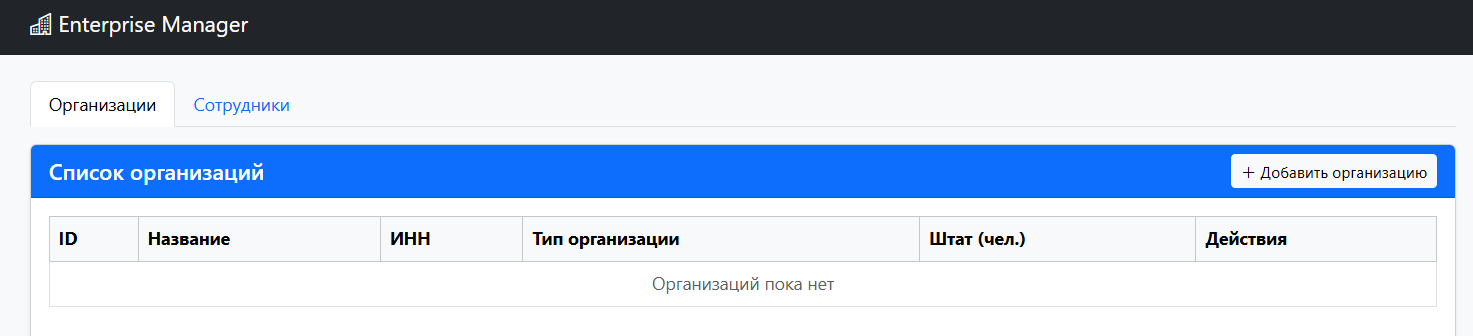
\includegraphics[width=0.8\textwidth]{организации.png}
  \caption{Экранная форма списка организаций}
  \label{fig:class_diagram_lab3}
\end{figure}

\begin{figure}[H]
  \centering
  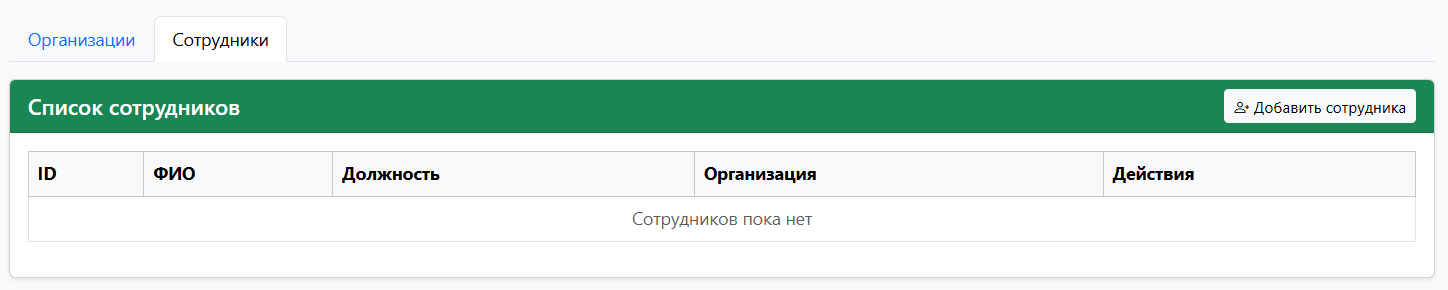
\includegraphics[width=0.7\textwidth]{сотрудники.png}
  \caption{Экранная форма списка сотрудников}
  \label{fig:class_diagram_lab3}
\end{figure}

\begin{figure}[H]
  \centering
  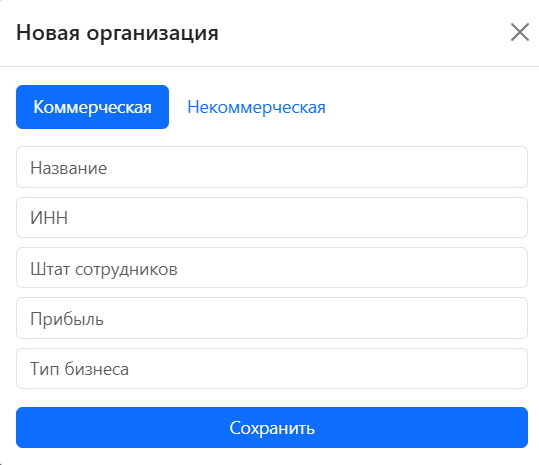
\includegraphics[width=0.8\textwidth]{добавление_комм.png}
  \caption{Экранная форма добавления коммерческих организаций}
  \label{fig:class_diagram_lab3}
\end{figure}

\begin{figure}[H]
  \centering
  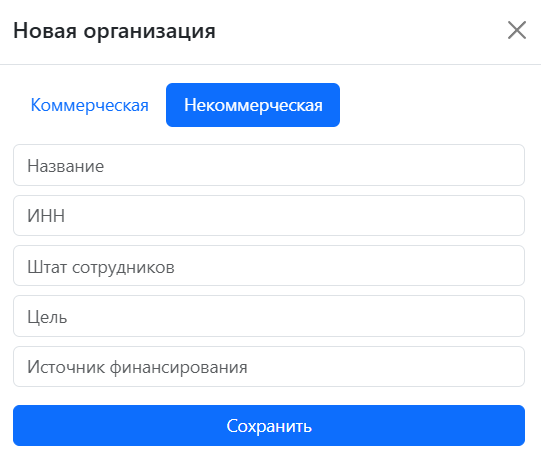
\includegraphics[width=0.8\textwidth]{добавление_некомм.png}
  \caption{Экранная форма добавления некоммерческих организаций}
  \label{fig:class_diagram_lab3}
\end{figure}

\begin{figure}[H]
  \centering
  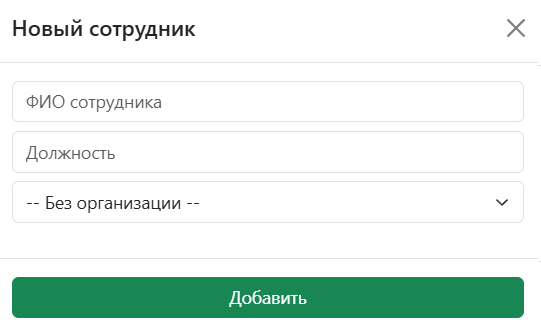
\includegraphics[width=0.8\textwidth]{добавление_сотрудник.png}
  \caption{Экранная форма добавления сотрудников}
  \label{fig:class_diagram_lab3}
\end{figure}

\newpage

\section*{Вывод}
\addcontentsline{toc}{section}{Вывод}

В ходе выполнения третьей лабораторной работы разработано веб-приложение на Java с использованием Spring Boot, Hibernate и PostgreSQL.

\begin{enumerate}
    \item Использован язык Java, сборщик Maven, СУБД PostgreSQL.
    \item Доступ к данным осуществляется через Hibernate  с помощью репозиториев, наследуемых CrudRepository.
    \item База данных содержит четыре таблицы, находящиеся в третьей нормальной форме. Реализована связь один ко многим между организациями и сотрудниками.
    \item Модель размечена аннотациями JPA используя Lombok.
    \item Веб интерфейс позволяет выполнять все CRUD-операции над организациями и сотрудниками.
\end{enumerate}

Приложение демонстрирует основные принципы ООП в контексте современного программирования на Java с использованием Spring.

\end{document}